\subsection{Increase number of scrambled datasets}
\label{lab:10K_scrambleddatasets}

%%%%%%%%%%%
%% Compare 1k and 10 results.
%% 1. create a table 
%% 2. Show plots

In this Section we comapred results across small and large sample sizes to study the  
impact of varying the number of scrambled datasets, 
as denoted by the sample size. We used two sample sizes, 1000 and 10000.
Table~\ref{table:scrambel_results_10K} shows fit results of two different sample size.
As we can see from the table that two set of results are consistent. Thus increasing number 
of scrambled datasets does not change results.

\begin{table}[hp]
    \begin{center}
    %%\resizebox{\textwidth}{!}{
    \begin{tabular}{|l|c|c|}
    \hline
    
    parameters & 1K & 10K \\ 
    \hline
    $d_{\it u}^{\it X,Z}$ & -2.98e-06 $\pm$ 3.68e-06& -2.99e-06 $\pm$ 3.62e-06\\
    \hline
    $d_{\it u}^{\it Y,Z}$ & -2.49e-06 $\pm$ 3.46e-06& -2.50e-06 $\pm$ 3.59e-06\\
    \hline
    $d_{\it u}^{\it XY,XY}$ & -1.62e-07 $\pm$ 1.86e-06& -2.39e-07 $\pm$ 1.89e-06\\
    \hline
    $d_{\it u}^{\it X,Y}$ & 1.05e-07 $\pm$ 9.27e-07& 1.41e-07 $\pm$ 9.40e-07\\
    \hline
    $c_{\it u}^{\it X,Z}$ & -2.31e-06 $\pm$ 2.86e-06& -2.32e-06 $\pm$ 2.81e-06\\
    \hline
    $c_{\it u}^{\it Y,Z}$ & -1.94e-06 $\pm$ 2.69e-06& -1.94e-06 $\pm$ 2.79e-06\\
    \hline
    $c_{\it u}^{\it XY,XY}$ & -1.26e-07 $\pm$ 1.45e-06& -1.86e-07 $\pm$ 1.47e-06\\
    \hline
    $c_{\it u}^{\it X,Y}$ & 8.17e-08 $\pm$ 7.20e-07& 1.09e-07 $\pm$ 7.31e-07\\
    \hline
    $c_{\it d}^{\it X,Z}$ & -1.03e-04 $\pm$ 1.27e-04& -1.03e-04 $\pm$ 1.25e-04\\
    \hline
    $c_{\it d}^{\it Y,Z}$ & -8.63e-05 $\pm$ 1.20e-04& -8.66e-05 $\pm$ 1.24e-04\\
    \hline
    $c_{\it d}^{\it XY,XY}$ & -5.59e-06 $\pm$ 6.45e-05& -8.27e-06 $\pm$ 6.54e-05\\
    \hline
    $c_{\it d}^{\it X,Y}$ & 3.64e-06 $\pm$ 3.21e-05& 4.86e-06 $\pm$ 3.25e-05\\
    \hline
    
    \hline
    \end{tabular}
    \end{center}
    \caption{Results from small and large number of scrambled datasets.
        Results are obtained using combined Run 2.
    }\label{table:scrambel_results_10K}
\end{table}







%%%%%%%%
%% Results of 10 batches
%%%%%%%%
%show ration table
To compete our studies, we split 10000 samples into 10 batches.
 Each batche contain 1000 scrabled datasets. In this study we comared
  results of 10 batches. Table of results of 10 batches
   is shown in the appendix~\ref{app:scrambled_10_batches}. 
The results in each batch is the average results obtained from 1000 fit results in
corresponding batch. Figure~\ref{fig:compare_10_batches} show the results 
 in each batch which is normalized to the result of first batch. The gray band in 
 the plot is the uncertainty band of the first batch. 
 From the plot we can see that results of 10 batches are consistent.

\begin{figure}[hp]
    \centering
    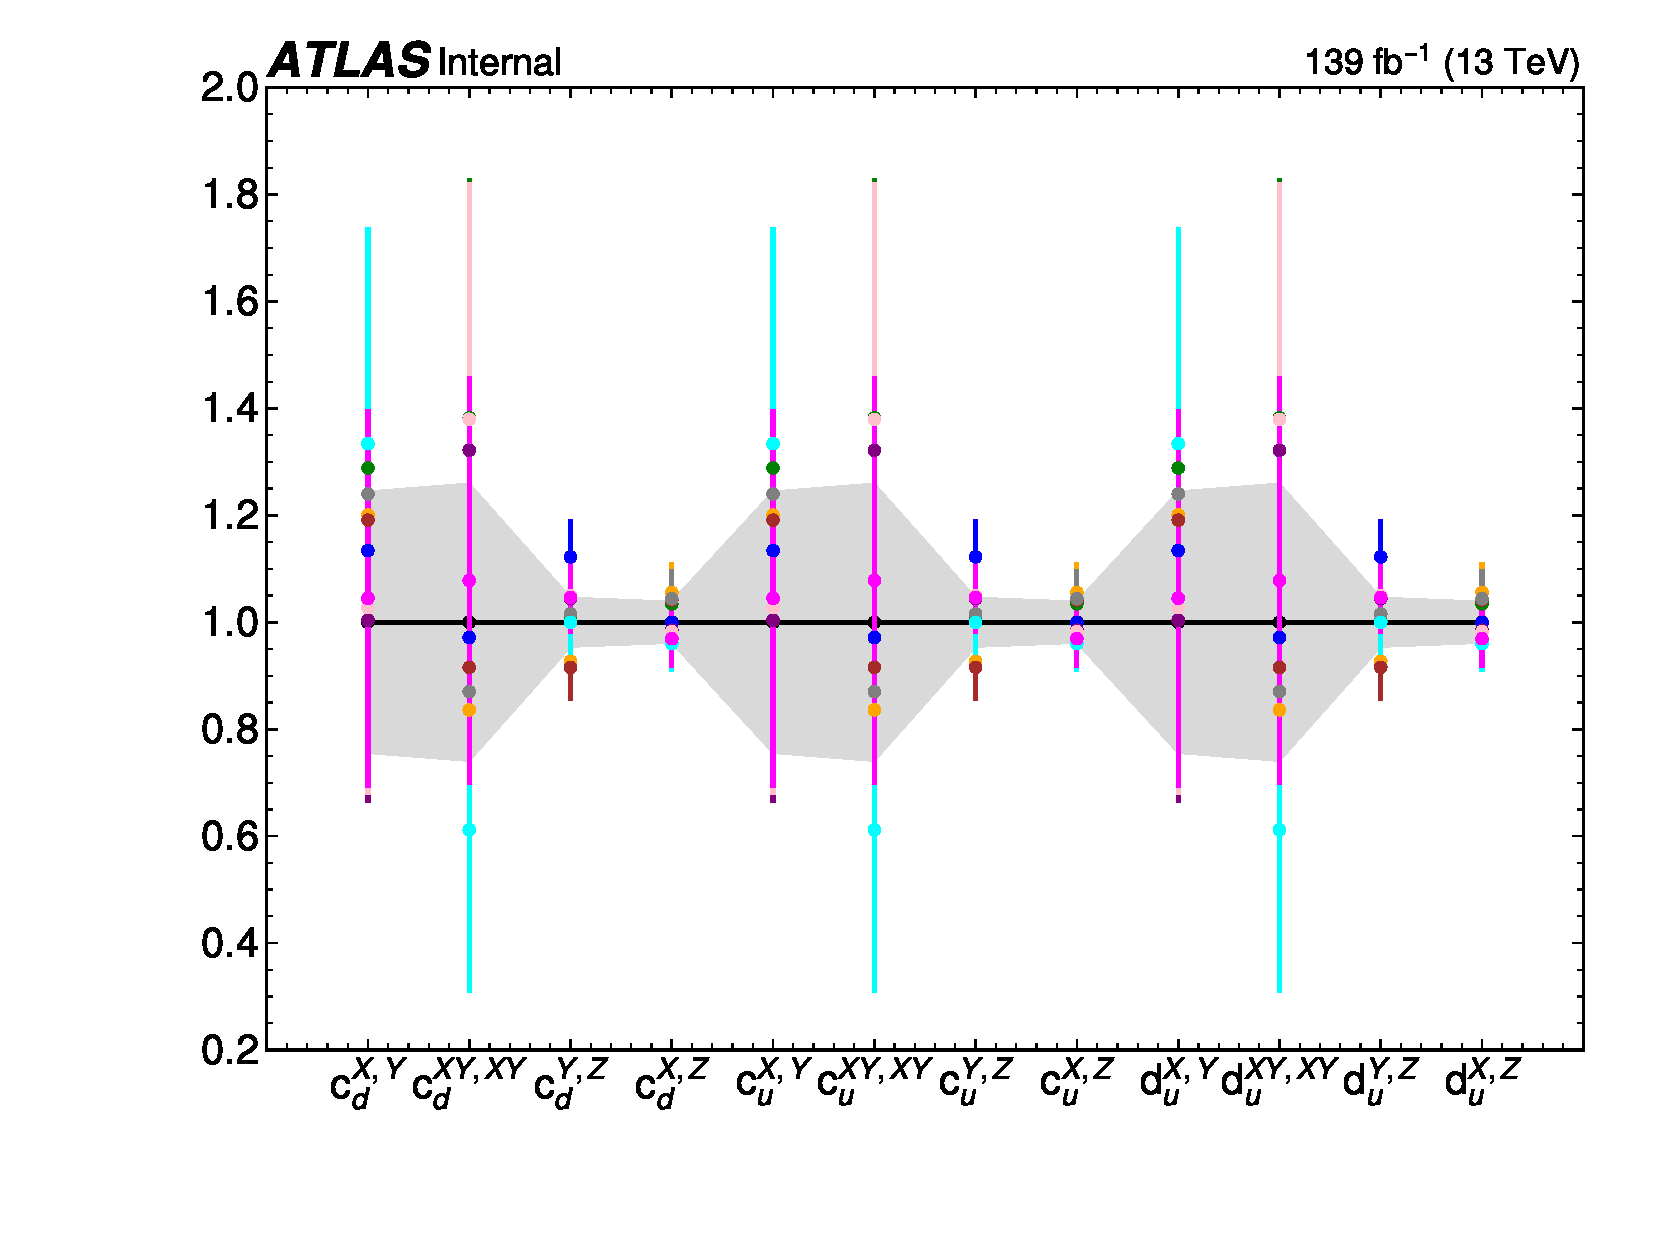
\includegraphics[width=0.45\textwidth]{figs/partially_unblinded_results/scrambled_10K/compare10K_results}
    \caption{The results in each batchs}
    \label{fig:compare_10_batches}
\end{figure}




\subsection{Investigate different probing periods}
\label{lab:scrambleddatasets_periods}

We checked scrambled datasets in various probing periods. As the results shown in
 Figure~\ref{fig:scrambled_Xperiods}, we didn't see any strange behavior in various periods.
 The 7 hours period showed slitly larger (compared to other periods) deviations from zeros. Therefore, we checked 6.87 and 7.13
 hours period to check if it is a coinsidence. The results of 6.87, 7, 7.13 hours periods show that 
 the slitly larger deviations is just a coinsidence (not related to a specific period).
\begin{figure}
    \centering
    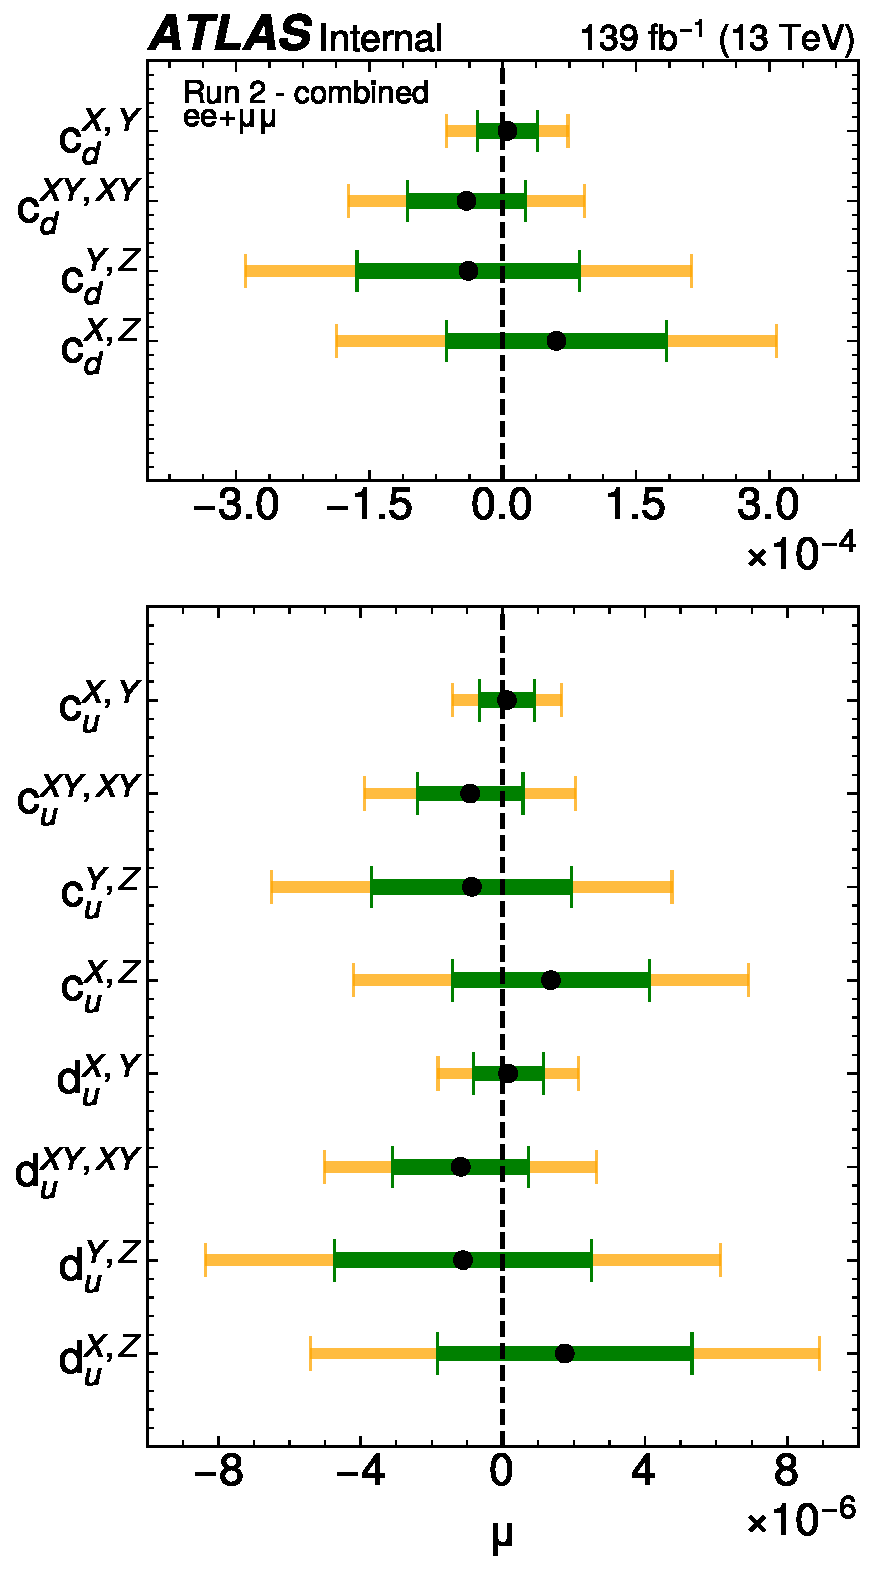
\includegraphics[ width=0.3\textwidth]{figs/partially_unblinded_results/periods/SigFit_summary_AllSamples_Combined_ll_1hour}
    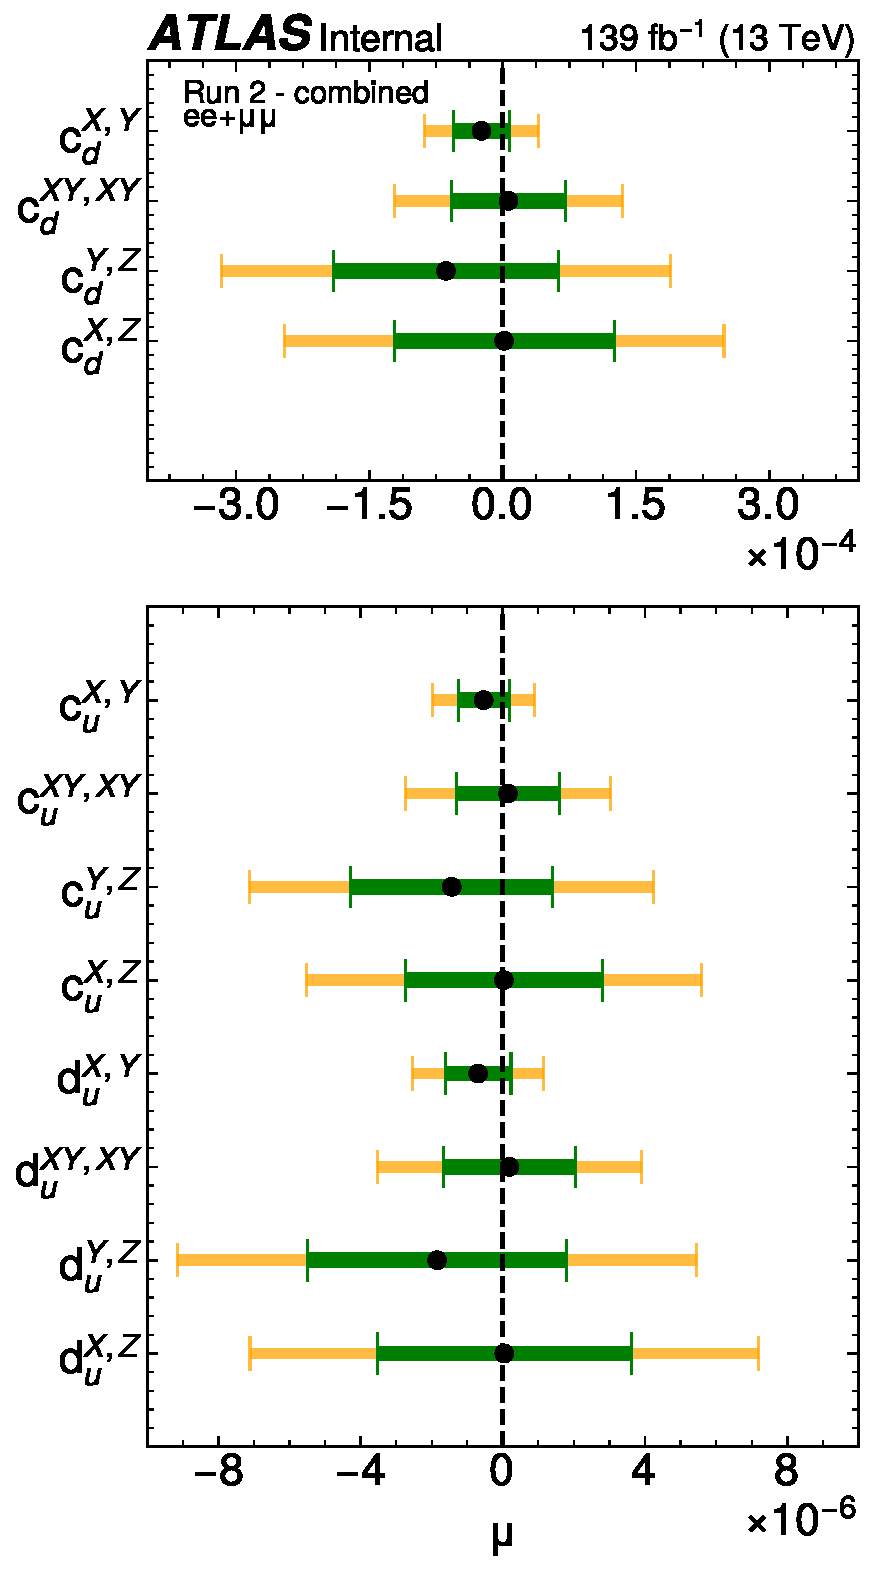
\includegraphics[ width=0.3\textwidth]{figs/partially_unblinded_results/periods/SigFit_summary_AllSamples_Combined_ll_24hour}
    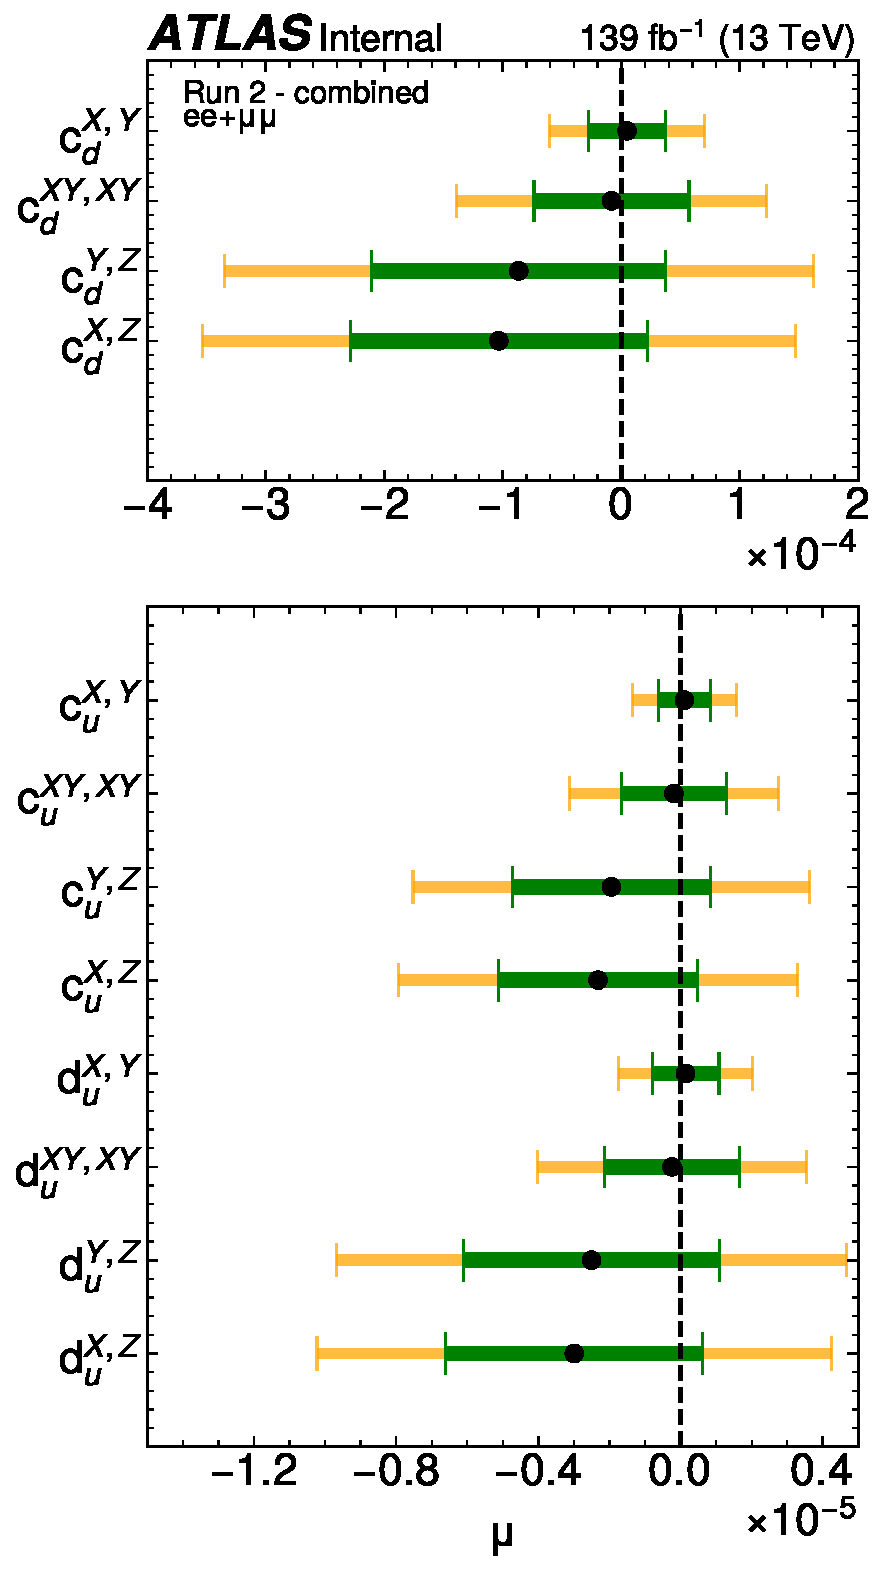
\includegraphics[ width=0.3\textwidth]{figs/partially_unblinded_results/periods/SigFit_summary_AllSamples_Combined_ll_sidereal_10K}\\
    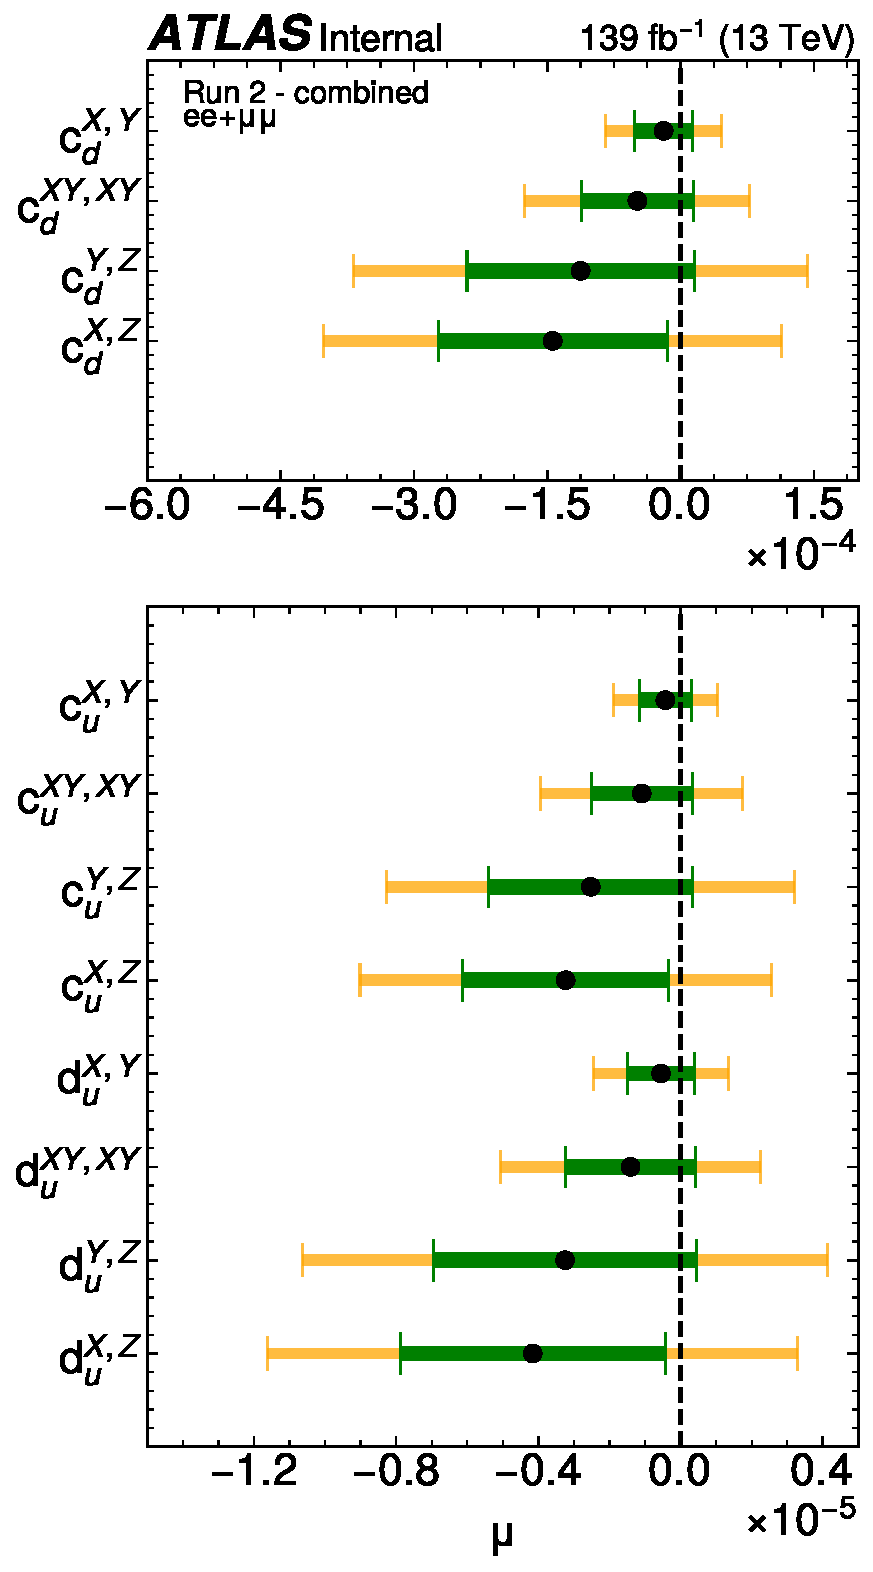
\includegraphics[ width=0.3\textwidth]{figs/partially_unblinded_results/periods/SigFit_summary_AllSamples_Combined_ll_6_87hour}
    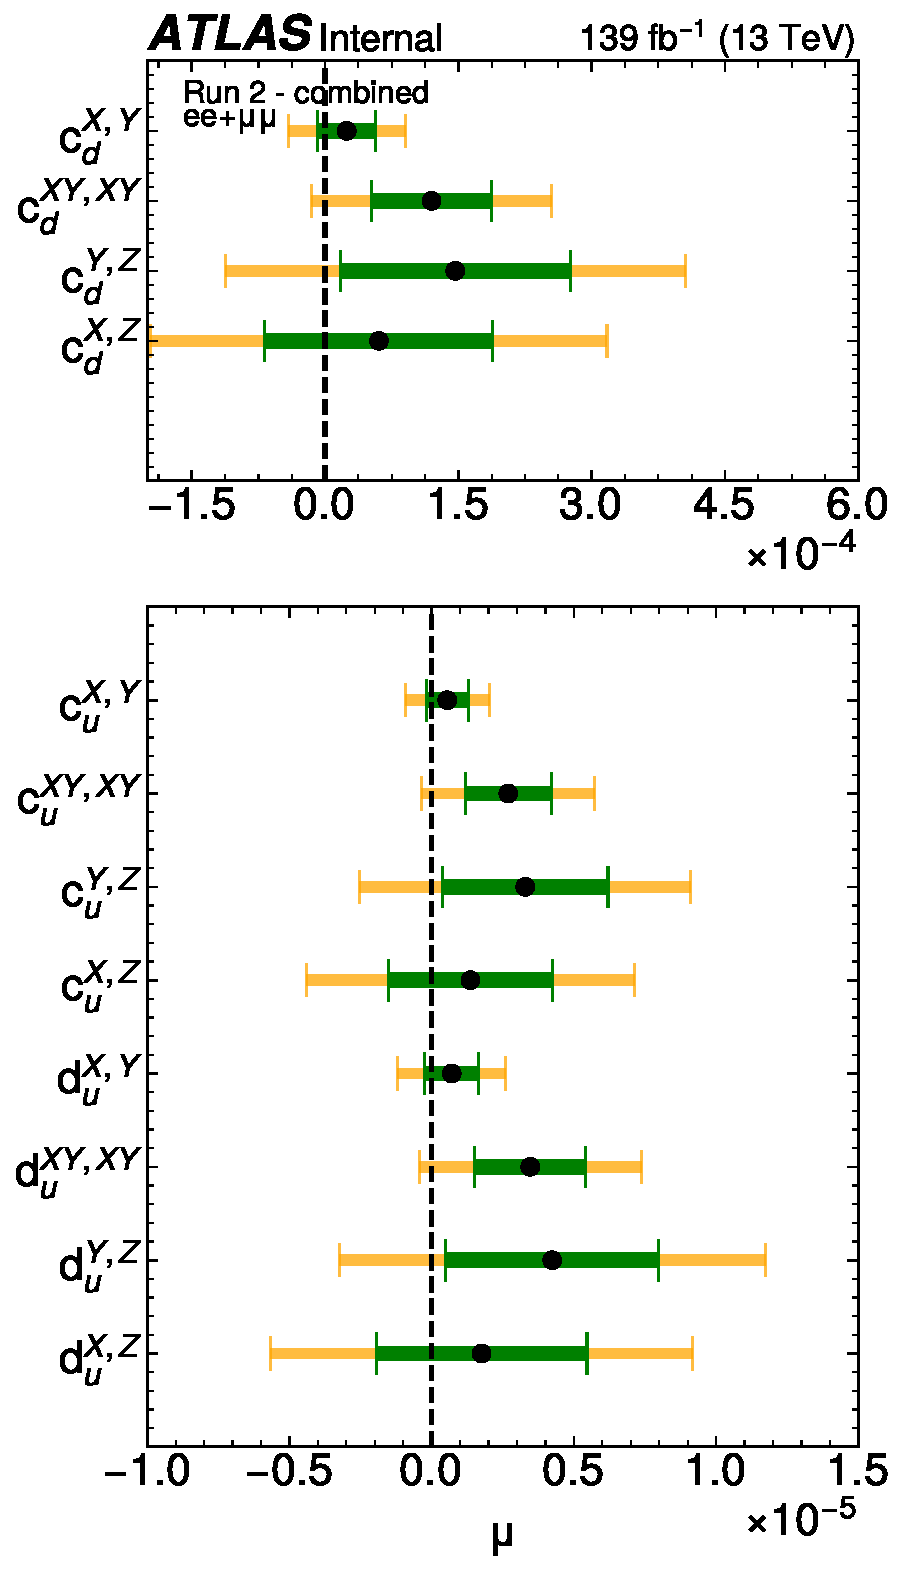
\includegraphics[ width=0.3\textwidth]{figs/partially_unblinded_results/periods/SigFit_summary_AllSamples_Combined_ll_7hour}
    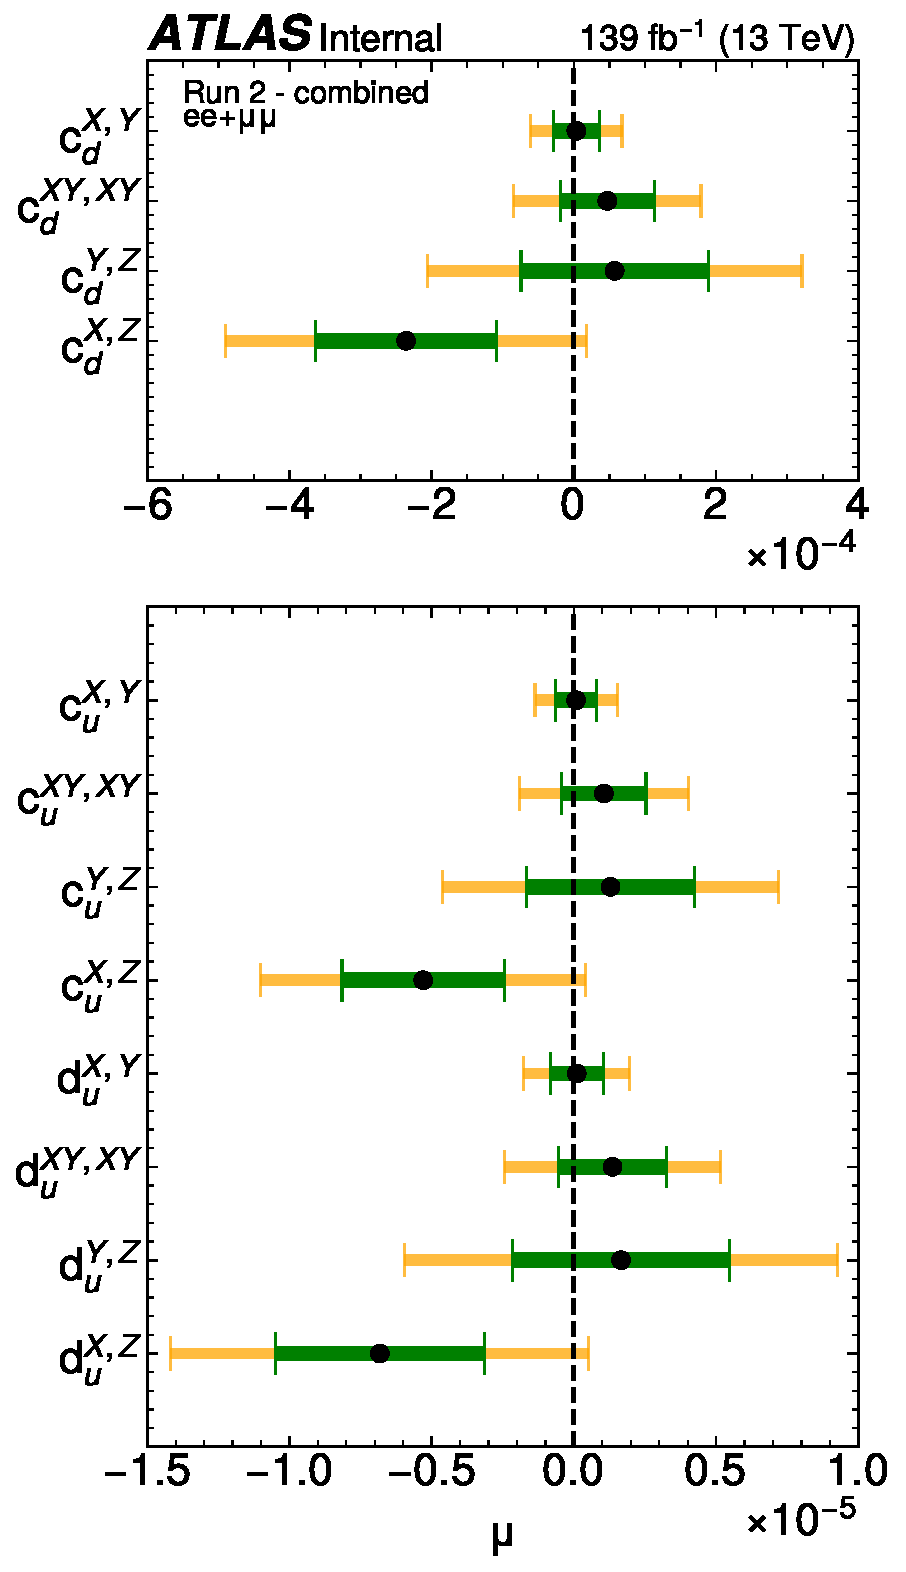
\includegraphics[ width=0.3\textwidth]{figs/partially_unblinded_results/periods/SigFit_summary_AllSamples_Combined_ll_7_13hour}

    \caption{Results of scrambled datasets in 1 hour (top left), 24 hours (top middle), 
    sidereal (top right), 6.87 hours (bottom left), 7 hours (bottom middle), and 
     7.13 hours (bottom right) periods. Results are the average of 1000 fit 
     results (the sidereal period used 10000 fit results).}
    \label{fig:scrambled_Xperiods}
\end{figure}



Figure~\ref{fig:scrambled_Xperiods_Spreads_Stats} shows Spreads VS average stats
 in 1, 6.87, 7, 7.13, 24 hours and sidereal periods. Detail of Spreads and Average Stats are described 
 in Section~\ref{sec:Spread_VS_Stats}.

\begin{figure}[hp]
    \centering
    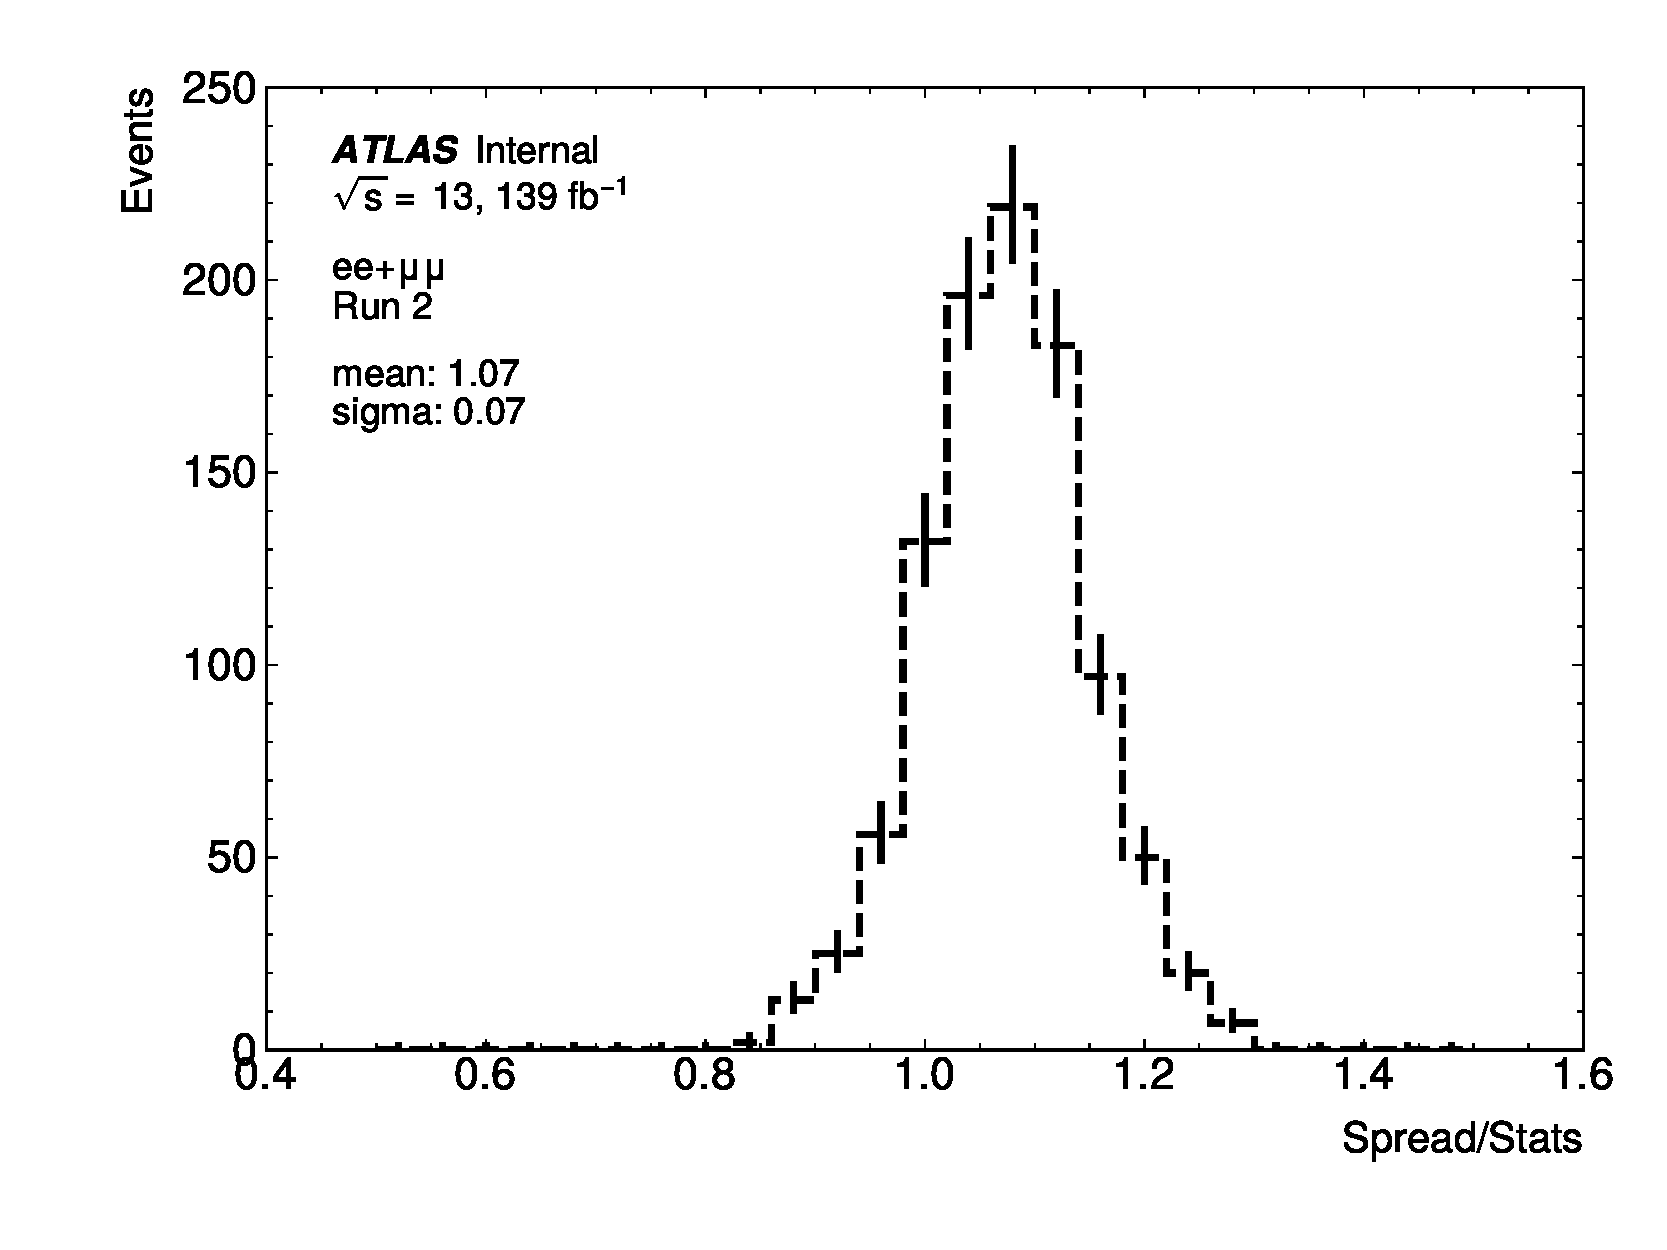
\includegraphics[width=0.3\textwidth]{figs/partially_unblinded_results/periods/spread_stats_scrambled_full_Ratio_1hour}
    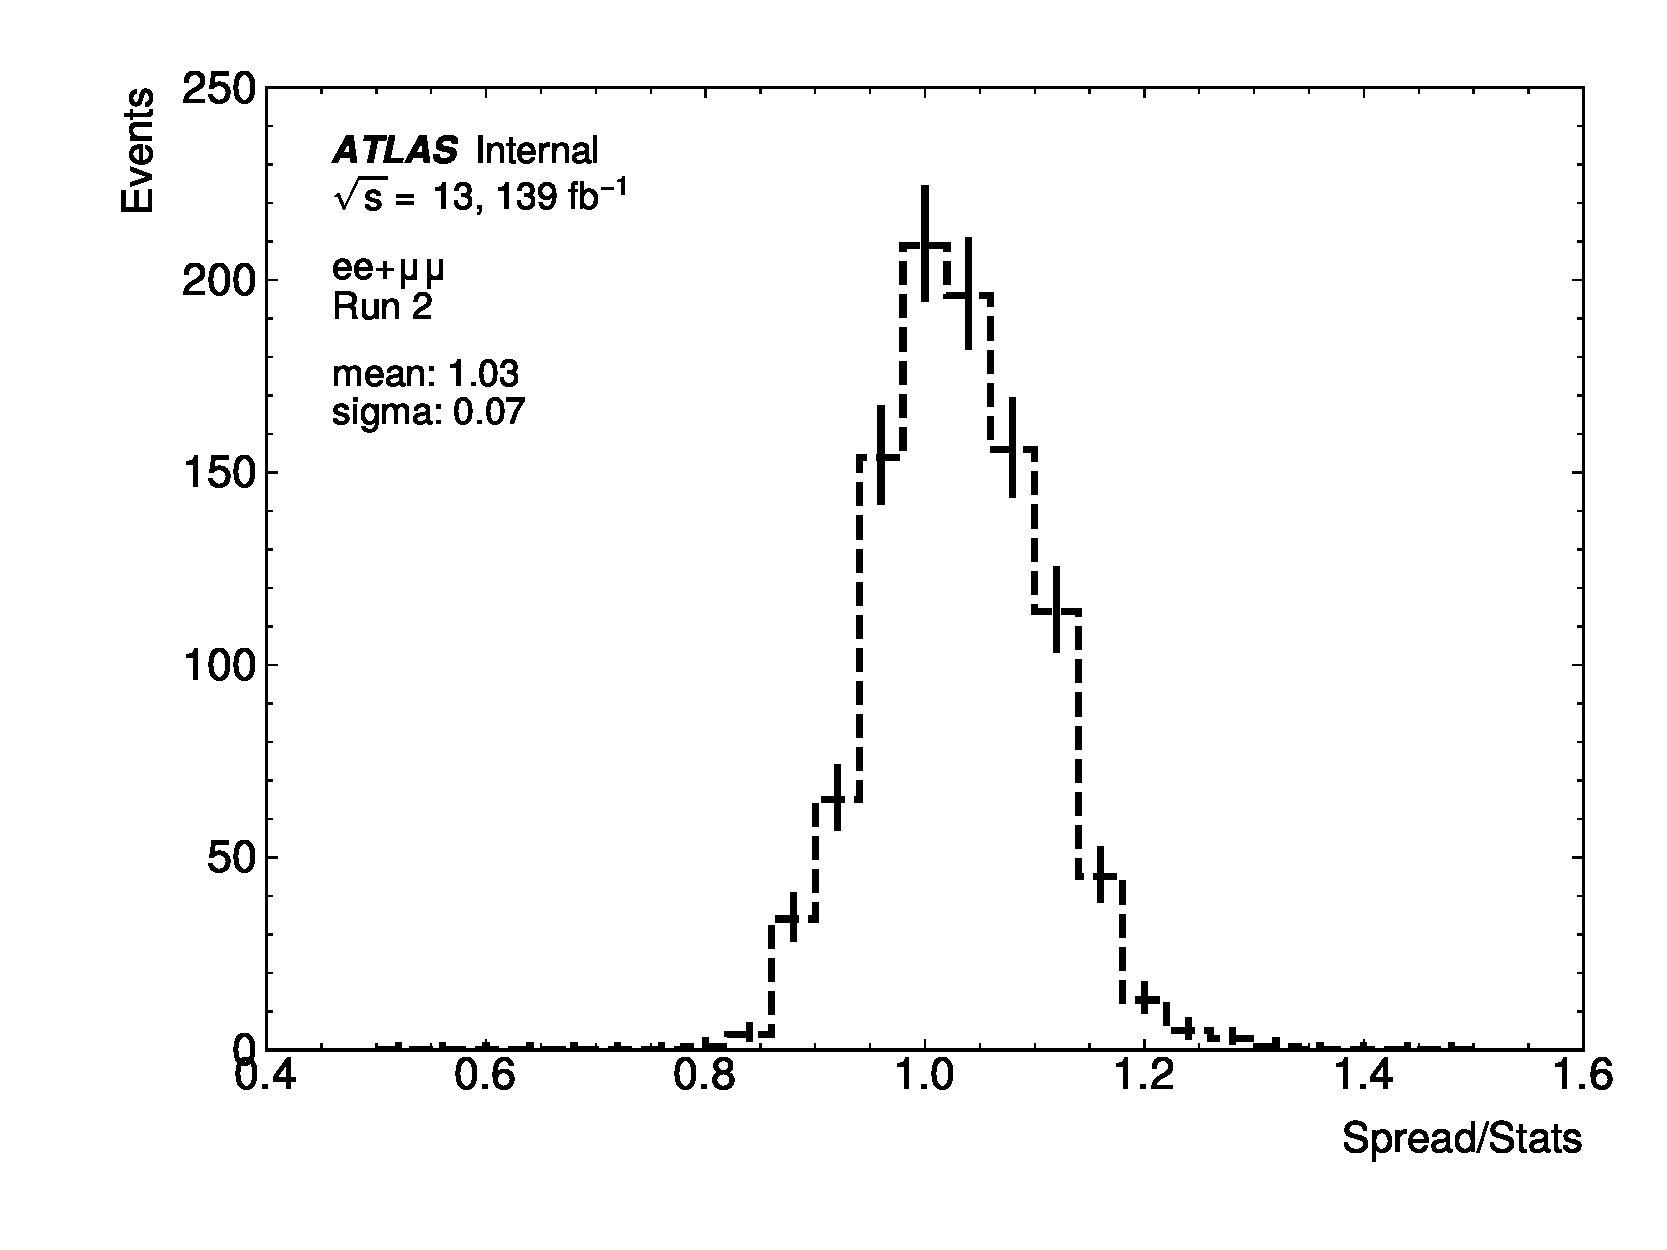
\includegraphics[width=0.3\textwidth]{figs/partially_unblinded_results/periods/spread_stats_scrambled_full_Ratio_6_87hour}
    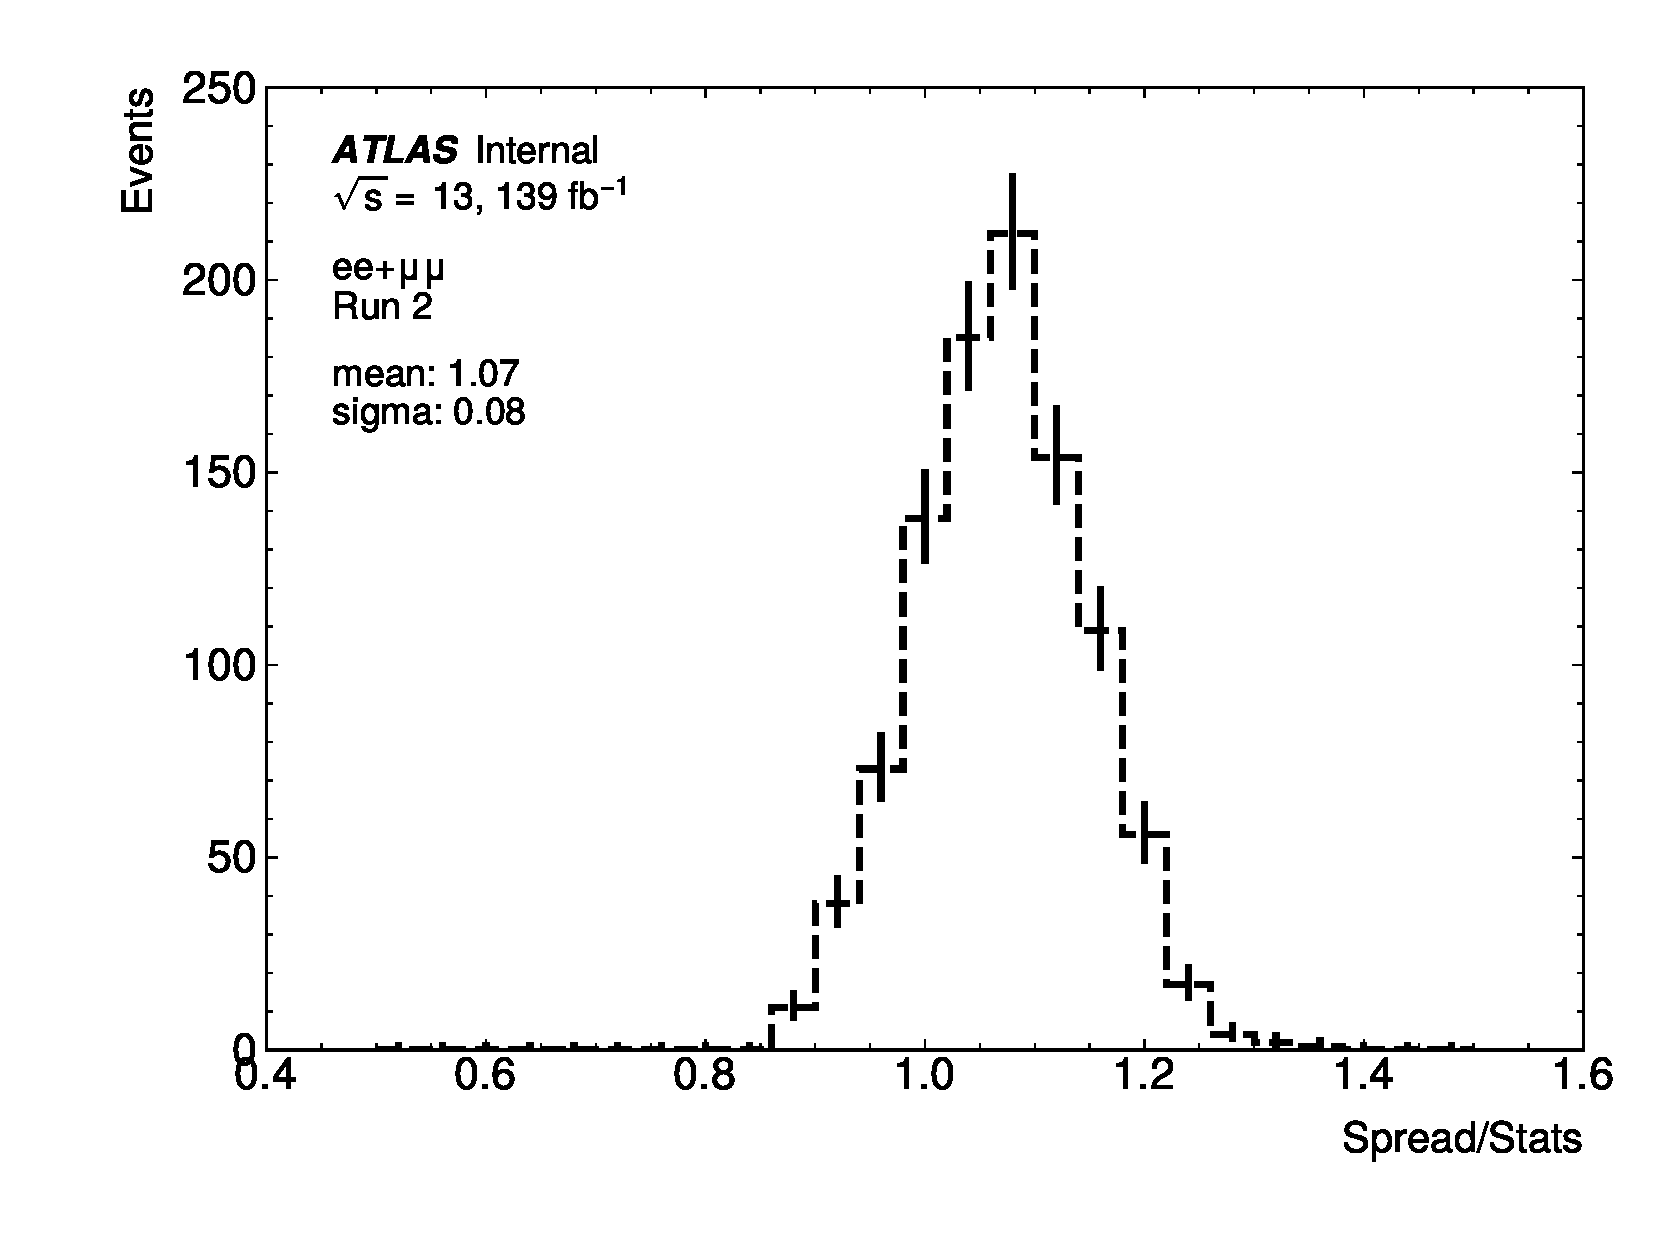
\includegraphics[width=0.3\textwidth]{figs/partially_unblinded_results/periods/spread_stats_scrambled_full_Ratio_7hour}\\
    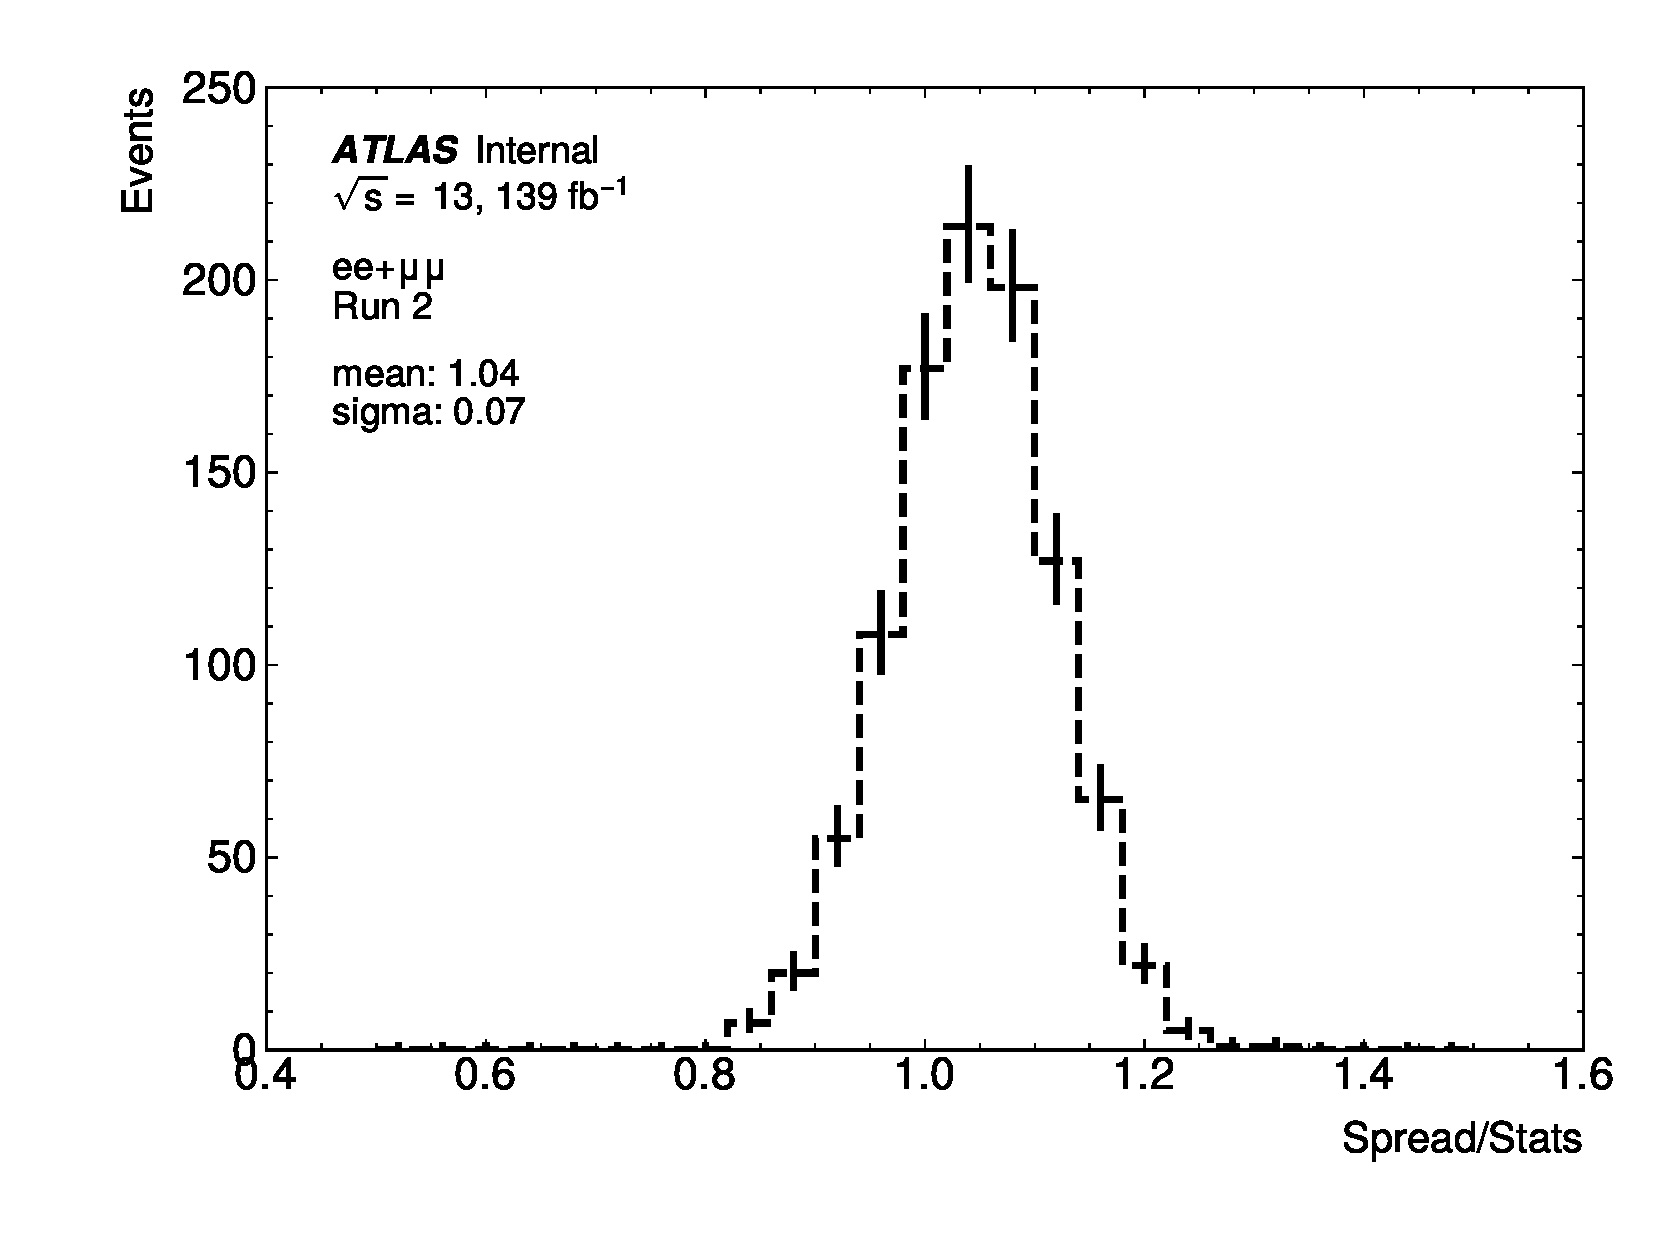
\includegraphics[width=0.3\textwidth]{figs/partially_unblinded_results/periods/spread_stats_scrambled_full_Ratio_7_13hour}
    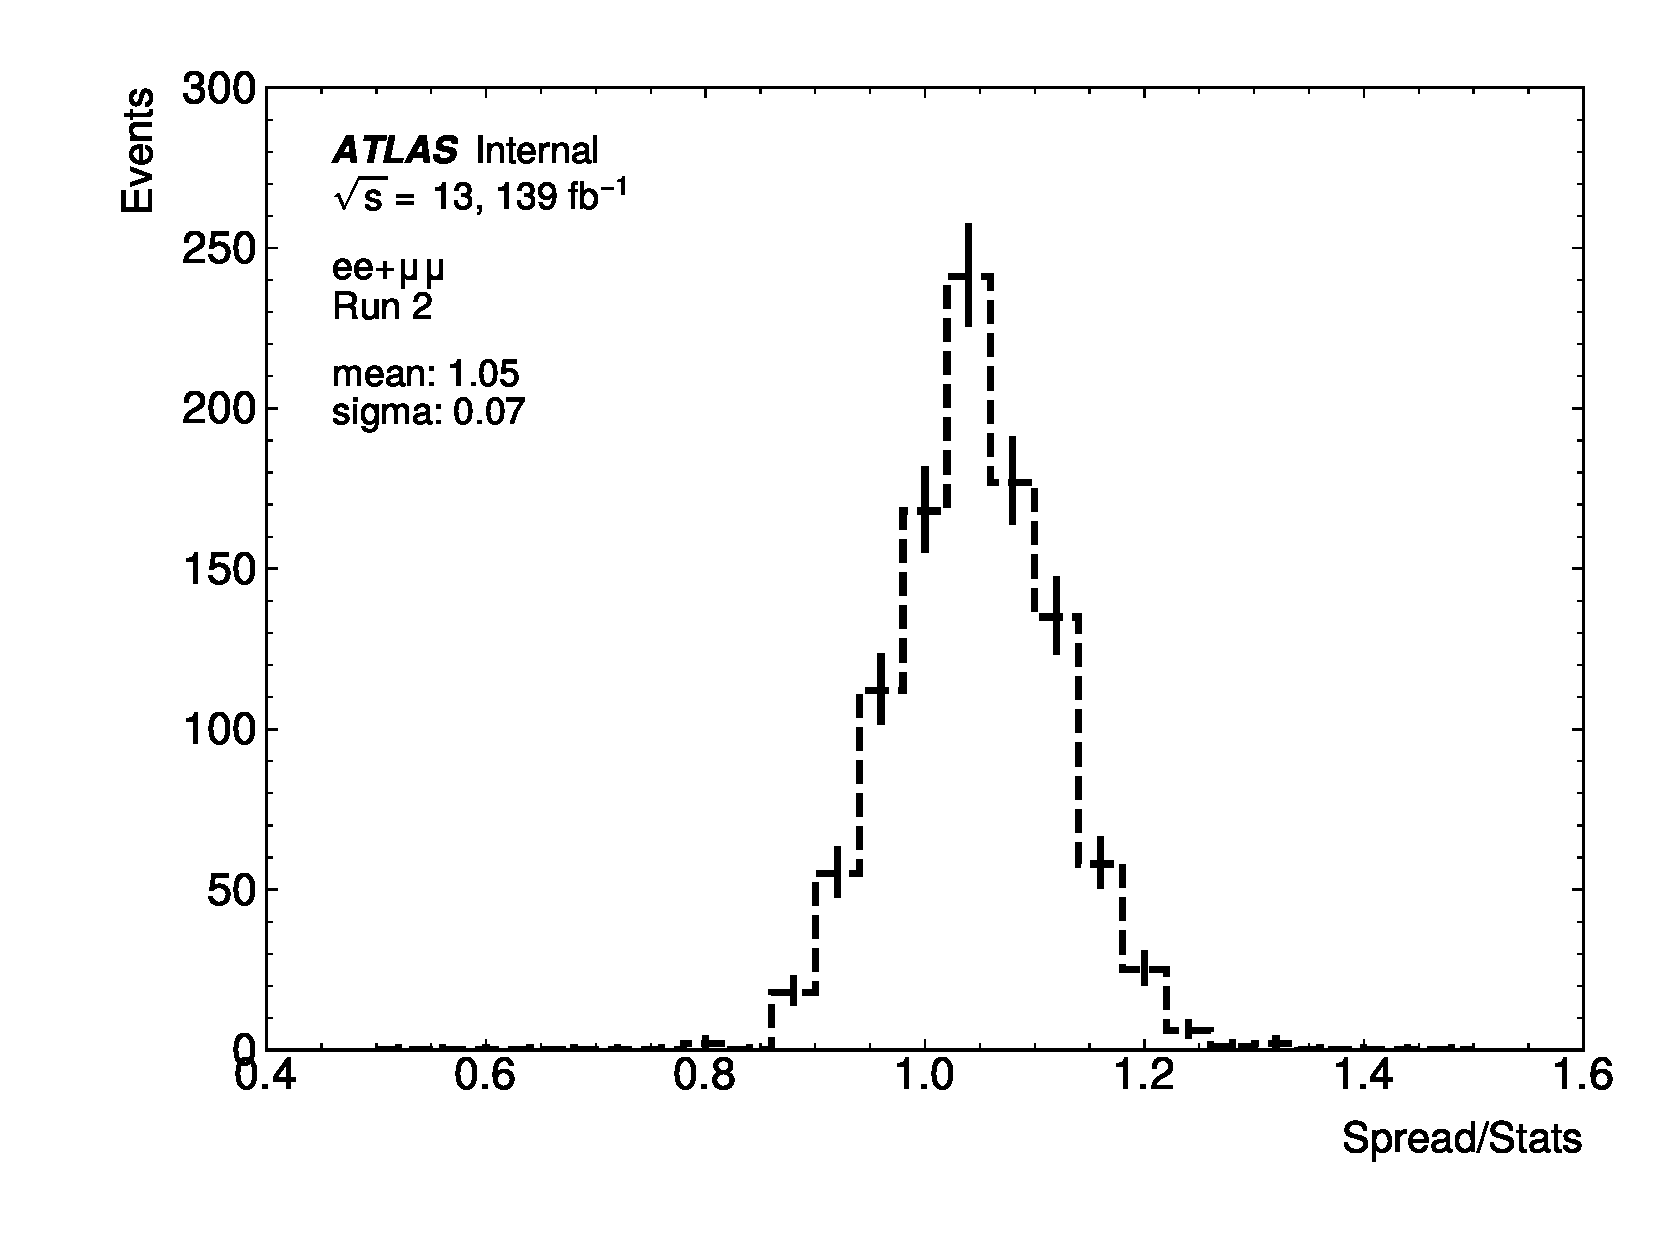
\includegraphics[width=0.3\textwidth]{figs/partially_unblinded_results/periods/spread_stats_scrambled_full_Ratio_24hour}
    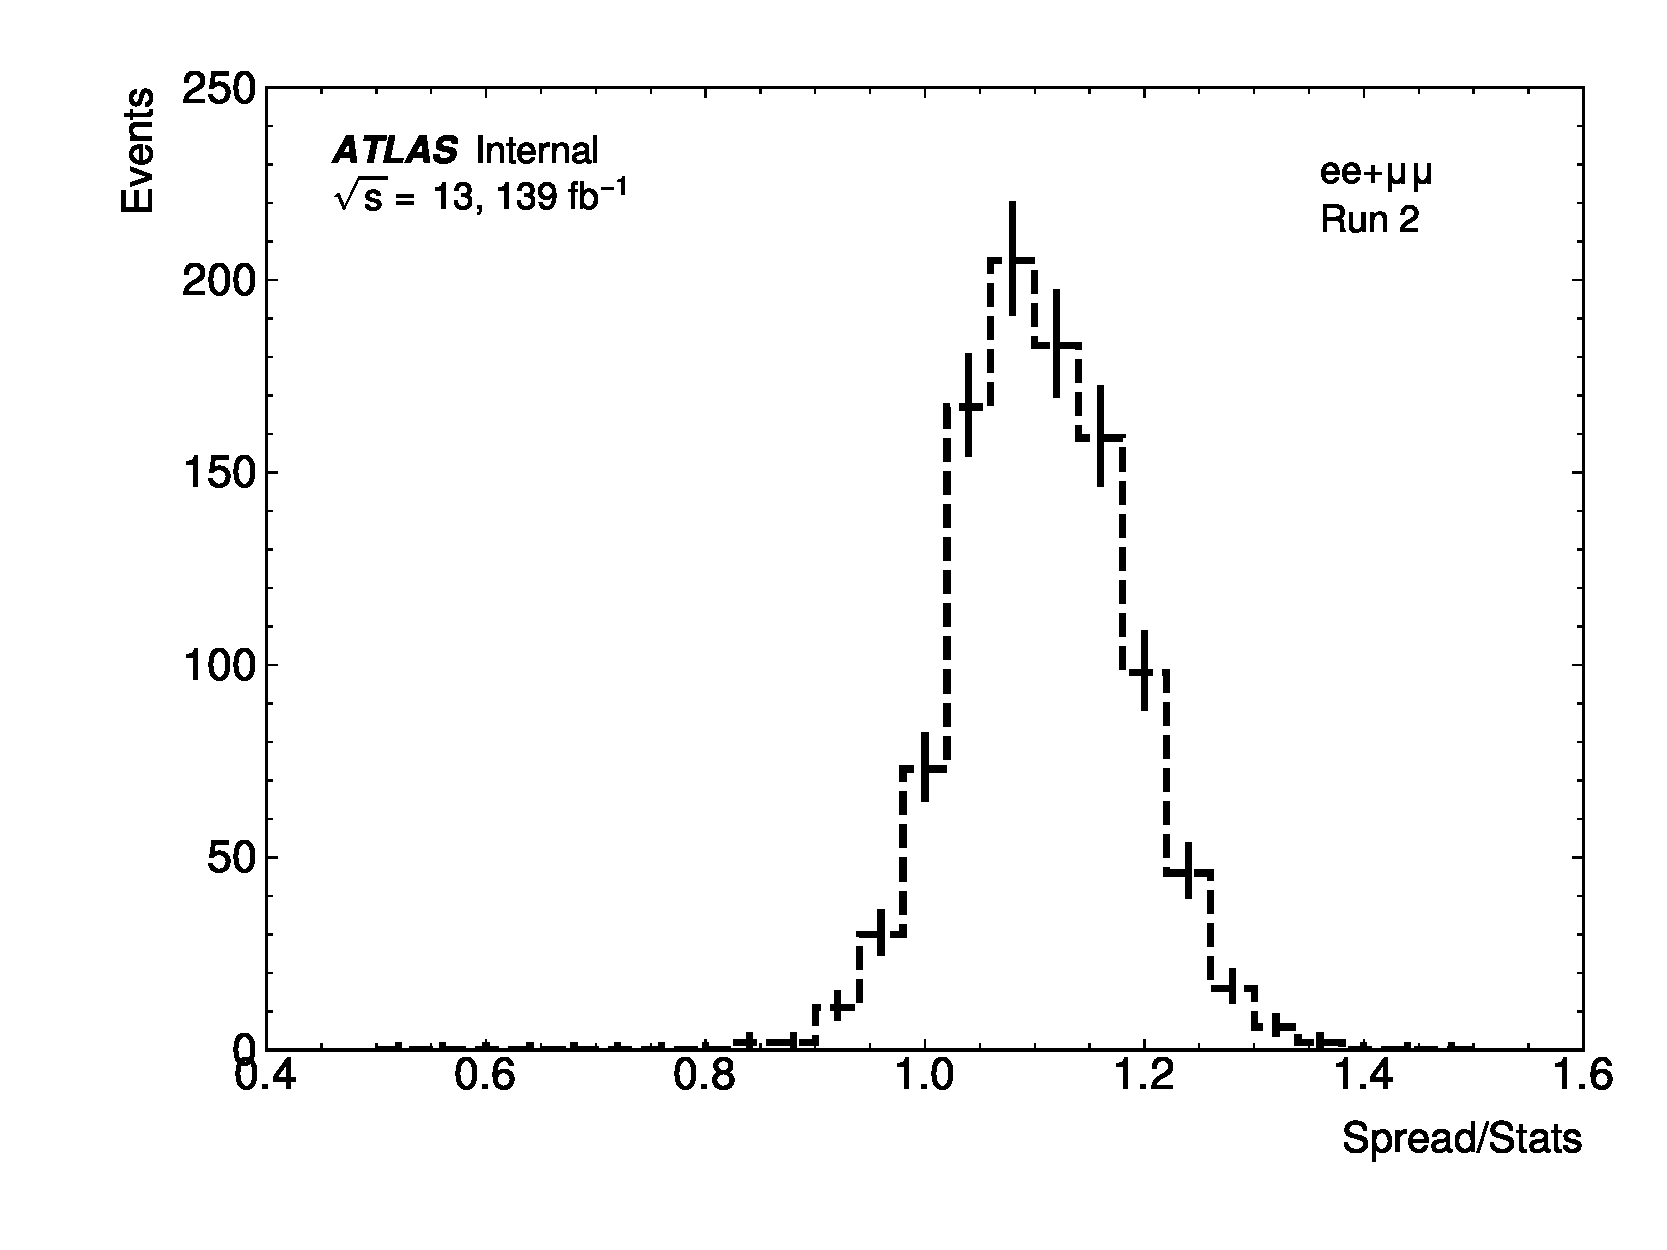
\includegraphics[width=0.3\textwidth]{figs/partially_unblinded_results/periods/spread_stats_scrambled_full_Ratio_sidereal}
    \caption{Left to right: 1, 6.87 and 7 hours perios (top plots); 7.13, 24 hours and sidereal perios (bottom plots).
    Spreads VS average stats. Plots show average results of 1000 scrambled datasets. 
    An average statistic is the average statistical uncertainty in each scrambled dataset, 
    and the spread of a dataset is an average of absolute residual.
    Spread is about 10-20\% larger in most of the scrambled datasets. This indicates there
     is a small systematic effect or the way we are calculating the ZC error in the double 
     ratio. This could be the reason why the average values shifted from zero}
    \label{fig:scrambled_Xperiods_Spreads_Stats}
    \end{figure}